\section{Implémentation}
\subsection{Environnement}
Nous avions au départ à notre disposition la Basys2 ainsi que le logiciel Xilinx et iSim pour visualiser les résultats de simulation. Afin de pouvoir avoir accès plus facilement à un FPGA et également profiter de plus de GPIOs et de mémoire nous avons acheté une DE0-Nano. Celle-ci étant un FPGA d'Altera, l'environnement de travail s'en est retrouvé changé. Nous sommes donc passé à Quartus pour le développement et la synthèse du code VHDL. De plus les IP cores diffèrent entre Xilinx et Quartus, nous avons donc dû effectuer quelques modifications au niveau de la ROM (utilisation du MegaWizard Manager de Quartus). Ayant rencontrés quelques problèmes avec Quartus, nous avons cependant continué à effectuer nos simulations à l'aide de Xilinx.\\

En ce qui concerne le matériel, nous avons utilisé une carte d'extension \cite{cite:vgaplus256kit} possédant entres autres un port VGA, un port PS/2 et un jack. La De0-Nano ne possédant pas de port VGA et de port PS/2, cela nous a permis d'interfacer un écran et un clavier à la carte.

\begin{figure}[h!]
	\centering
	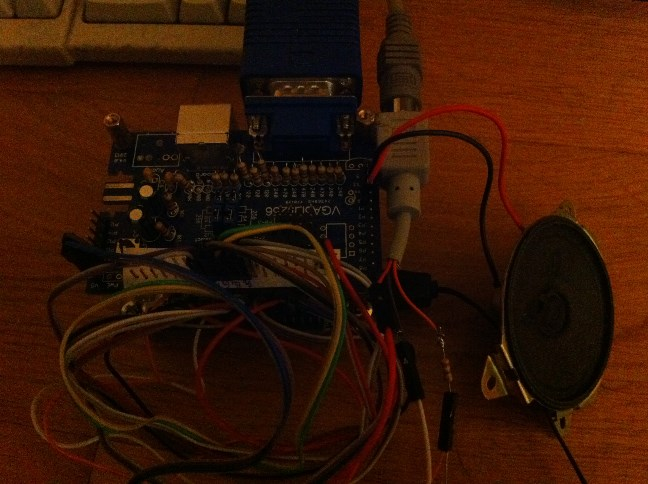
\includegraphics[scale=0.5]{images/IMG_1017.jpg}
	\caption{Photo de la DE0-Nano avec la carte d'extension fixée au dessus}
	\label{fig:photoDE0}
\end{figure}

\newpage
\subsection{Conventions}
Afin d'avoir une certaine cohérence entre nos différentes entités, nous avons essayé de respecter certaines conventions. Nous avons tout d'abord limiter l'utilisation de generics aux entités nécessitant de multiples instanciations, et d'utiliser des constantes contenus dans des packages (\emph{kbd\_pkg}, \emph{vga\_pkg}, \emph{game\_pkg}) dans les autres cas. Si nous avions utiliser des generics dans toutes les entités et avions seulement déclarés des constantes dans l'entité  \emph{pong} (top entity), nous aurions été forcé de cascader les generics ce qui devient vite contraignant.\\

Nous avons également utilisé \emph{open} afin de laisser vide des signaux de sorties dont nous ne nous servions pas lors d'instanciation d'entités. Pour les constantes et generics nous avons opté pour des majuscules, et pour les signaux des minuscules. les mots contenus dans les noms d'entités/signaux/constantes ont été séparés par des underscores ("\_"). De plus, lorsque cela était possible, nous avons utilisé la boucle \emph{for generate} afin de garder un code clair.

\newpage
\subsection{Génération signaux VGA}
\begin{figure}[h!]
	\centering
	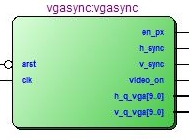
\includegraphics{images/vgasync.jpg}
	\caption{Schéma entité vgasync}
	\label{fig:vgasync}
\end{figure}

Ayant ajouté une carte d'extension utilisant des DACs 3 bits pour le rouge, 3 bits pour le vert, et 2 bits pour le bleu, nous avons généré nos couleurs sur 8 bits, soit 256 possibilités de couleurs. Nous avons également généré les signaux de synchronisation \emph{h\_sync} et \emph{v\_sync}.\\

D'après le tableau des timings du VGA\cite{cite:timingsvga}, pour une résolution de 640x480 60Hz la vitesse à laquelle doit être parcourue les pixels doit être d'environ 25 MHz. Pour cela nous avons instancié l'entité clkdiv ayant un enable (\emph{enclk}) en sortie permettant de faire fonctionner les autres blocs à une fréquence plus faible que celle de l'horloge.\\

Nous devons parcourir l'écran pixel par pixel, pour cela nous avons instancié deux compteurs (entité \emph{cnt}), un pour la position horizontale et l'autre pour la position verticale des pixels, comptant de 0 jusqu'à \emph{active zone} + \emph{back porch} + \emph{sync pulse} + \emph{front porch}. Ces compteurs sont autorisés à compter lorsque \emph{en\_px}  est à 1 (signal d'enable permettant de parcourir les pixels à 25 MHz). Lorsque le compteur horizontal arrive à sa valeur max, le signal \emph{maxed} du compteur passe à 1 et est relié à l'entrée \emph{cnten} du compteur vertical afin de l'autoriser à s'incrémenter, le compteur vertical s'incrémente donc à chaque fois qu'une ligne est parcourue.\\

Pour générer les signaux \emph{h\_sync} et \emph{v\_sync}, nous devons les mettre à l'état bas (actif) lorsque les compteurs \emph{h\_q\_int} et \emph{v\_q\_int} sont dans la zone de \emph{sync pulse}. Cela revient donc aux conditions suivantes :
\begin{flalign*}
&\text{\textbf{horizontal état bas (actif)}}&\\
&h\_q\_int >= H\_AT + H\_FP&\\
&\text{and } h\_q\_int < H\_AT + H\_FP + H\_SP&\\\\
&\text{\textbf{vertical état bas (actif)}}&\\
&v\_q\_int >= V\_AT + V\_FP&\\
&\text{and } v\_q\_int < V\_AT + V\_FP + V\_SP&
\end{flalign*}
Avec \emph{x\_q\_int} compteur de pixels \textbf{h}orizontal/\textbf{v}ertical\\
\emph{X\_AT} zone active horizontale/verticale\\
\emph{X\_FP} front porch horizontal/vertical\\
\emph{X\_BP} back porch horizontal/vertical\\
\emph{X\_SP} sync pulse horizontal/vertical\\

\newpage
Nous avons également généré un signal \emph{video\_on} actif lorsque les compteurs de pixels horizontal et vertical sont dans leur zone active respective.
\begin{flalign*}
&\text{\textbf{Conditions nécessaires pour \emph{video\_on} à l'état haut (actif)}}&\\
&h_q\_int < H\_AT&\\
&\text{and } v\_q\_int < V\_AT&
\end{flalign*}

\newpage
\subsection{Utilisation de la ROM}
La De0-Nano possède de la RAM utilisable à l'aide de blocs paramétrables dans Quartus II (Intellectual Property Blocks). L'outil MegaWizard Plug-In Manager (Tools -> MegaWizard Plug-In Manager) permet de créer des entités donnant accès à différents types de mémoires (RAM: 1-PORT, ROM:1-PORT, etc).\\

\begin{figure}[h!]
	\centering
	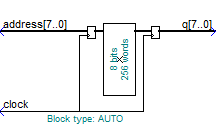
\includegraphics{images/romschem.png}
	\caption{Schéma ROM contenant 256 adresses et 8 bits de sortie}
	\label{fig:romschem}
\end{figure}

Nous souhaitons créer une ROM: 1-PORT contenant des images à afficher sur l'écran. Celle-ci comporte 2 entrées, horloge et adresse, et une sortie. La taille du bus d'adresse et de sortie doivent être précisées. La dernière étape est l'indication d'un fichier \emph{mif} décrivant le contenu de la ROM. Celle-ci nécessite les informations suivantes :
\begin{description}
\item[Depth] indique la taille du bus d'adresses
\item[Width] indique la taille du bus de sortie
\item[Address radix] base utilisée pour les adresses
\item[Data radix] base utilisée pour les données
\item[Content] Contenu de la ROM sous la forme \emph{adresse : donnée;}
\end{description}

Nous avons généré deux ROMs, l'une contenant un jeu de caractère (noir et blanc), et l'autre contenant une image à afficher en fond ($95*128$, 8 bits de couleurs). Pour générer le fichier \emph{mif} correspondant à ces images, une fonction MATLAB \cite{cite:rommatlab} a été utilisée pour générer un fichier \emph{mif}, puis un traitement simple a été effectué pour rajouter des adresses associées à la donnée \emph{0x00} afin d'atteindre une puissance de 2.\\

\noindent \textbf{N.B.} Le code ci-dessous correspond à la fonction permettant de convertir une image ayant des couleurs sur 8 bits. Pour une image ne possédant qu'un seul bit de couleur (noir ou blanc) la fonction a été modifiée.\\

\begin{lstlisting}
function img2 = IMG2mif8(imgfile, outfile)

img = imread(imgfile);
height = size(img, 1);
width = size(img, 2);
s = fopen(outfile,'wb');

% header
fprintf(s,'DEPTH = %d;\n', height*width);
fprintf(s,'WIDTH = 8;\n');
fprintf(s,'ADDRESS_RADIX = UNS;\n');
fprintf(s,'DATA_RADIX = HEX;\n');
fprintf(s,'CONTENT\n');
fprintf(s,'BEGIN\n');

% content
cnt = 0;
cntadr = 0;
img2 = img;
for r=1:height
    for c=1:width
        cnt = cnt + 1;
        R = img(r,c,1);
        G = img(r,c,2);
        B = img(r,c,3);
        Rb = dec2bin(R,8);
        Gb = dec2bin(G,8);
        Bb = dec2bin(B,8);
        img2(r,c,1) = bin2dec([Rb(1:3) '00000']);
        img2(r,c,2) = bin2dec([Gb(1:3) '00000']);
        img2(r,c,3) = bin2dec([Bb(1:2) '000000']);
        Outbyte = [ Rb(1:3) Gb(1:3) Bb(1:2) ];
        if (Outbyte(1:4) == '0000')
            fprintf(s,'%d : 0%X',cntadr, bin2dec(Outbyte));
        else
            fprintf(s,'%d : %X',cntadr, bin2dec(Outbyte));
        end
        
        fprintf(s,';\n');
        cntadr = cntadr + 1;
    end
end

fprintf(s,'END;');

fclose(s);
\end{lstlisting}

\begin{figure}[h!]
	\centering
	\begin{subfigure}[b]{0.1\textwidth}
		\centering
		
\includegraphics[width=\textwidth]{images/cirno2.jpg}
		\label{fig:cirno2}
	\end{subfigure}
	~

	\begin{subfigure}[b]{0.4\textwidth}
		\centering
		
\includegraphics[width=\textwidth]{images/pixelfont.jpg}
		\label{fig:pixelfont}
	\end{subfigure}
	\caption{Images contenues dans la ROM}
\end{figure}


\begin{figure}[h!]
	\centering
	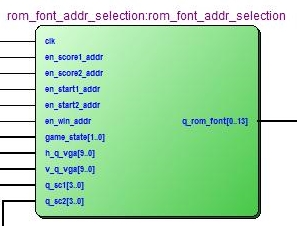
\includegraphics[scale=1.0]{images/romfontaddr.jpg}
	\caption{Schéma entité rom\_font\_addr\_selection}
	\label{fig:romfontaddr}
\end{figure}
La sélection d'adresses pour la ROM contenant le jeu de caractères se fait au niveau de l'entité \emph{rom\_font\_addr\_selection}. Celle-ci prend en entrée un enable pour les différentes zones dans lesquelles le contenu de la ROM doit être affiché. Cette enable doit se produire un cycle d'horloge avant l'affichage dans la zone désirée, en effet le bloc de ROM dépend de l'horloge, et lorsqu'une adresse entre dans celui-ci la sortie est disponible au coup d'horloge suivant.\\

Une fois l'adresse sélectionnée, pour récupérer la sortie nous pouvons utiliser le compteur de position horizontal (valeur du compteur horizontal - position horizontale du caractère à afficher), ce qui nous permet de récupérer les bits un par un afin de définir ou non une couleur spécifique pour le pixel actuellement parcouru.\\

Pour générer l'image de fond, le principe diffère légèrement. En effet pour une adresse donnée, la sortie de \emph{rom\_bg} est la couleur d'un pixel. Pour adresser chaque pixel il faudrait donc multiplier les deux signaux de compteurs de pixels (horizontal et vertical). Pour éviter cela, un compteur supplémentaire a été crée afin de compter à la vitesse de la pixel clock lorsque les compteur de pixels se trouvent dans la bonne zone.

\newpage
\subsection{Utilisation du clavier}
\begin{figure}[h!]
	\centering
	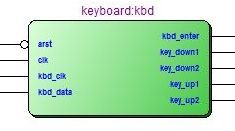
\includegraphics[scale=1.0]{images/kbdentity.jpg}
	\caption{Schéma entité keyboard}
	\label{fig:kbdentity}
\end{figure}

La gestion du clavier se fait à l'aide de l'entité \emph{keyboard}. Celle-ci prend en entrée les signaux \emph{kbd\_clk}, signal d'enable généré par le clavier permettant d'indiquer lorsqu'une donnée est reçue, et \emph{kbd\_data}, signal permettant de recevoir les données en série. Les signaux de sortie indiquent l'état d'une touche du clavier, \emph{key\_up1}, \emph{key\_down1}, \emph{key\_up2}, \emph{key\_down2} et \emph{key\_enter} correspondant respectivement aux touches A, Q, Z, S et ENTRÉE du clavier.\\

Lorsqu'une donnée est disponible sur le signal \emph{kbd\_data}, le signal \emph{kbd\_clk} passe à l'état bas (actif). Nous devons donc détecter un front descendant sur ce dernier en comparant sa valeur actuelle et son ancienne valeur \emph{kbd\_clk\_old}. Pour cela nous assignons la valeur de \emph{kbd\_clk} à \emph{kbd\_clk\_old} lorsqu'un coup d'horloge intervient. Les données sont ensuite récupérées une par une à l'aide d'un registre à décalages Serial-In Parallel-Out, \emph{data\_shift}. Les 8 bits de données peuvent être récupérés sur le signal \emph{data} lorsque le bit de start atteint le LSB de \emph{data\_shift} (initialement rempli de '1'). Une fois une donnée disponible, celle-ci est comparée aux codes correspondant aux touches qui nous intéressent pour savoir si le signal correspondant doit passer à l'état actif ou non. Pour vérifier le relâchement d'une touche, l'ancienne valeur contenue dans data est stockée dans \emph{old\_data}, ce qui permet de vérifier si le code relâchement a été envoyé et avec quel code de touche celui-ci a été envoyé.

\newpage
